% !TeX program = xelatex
% Standalone: only the unit10 sampling-distribution figure (export to PNG for site)
\documentclass[tikz,border=2pt]{standalone}
\usepackage{fontspec}
\newfontfamily\figurelatinfont{Times New Roman}
\usepackage{pgfplots}
\pgfplotsset{compat=1.18}
\usepgfplotslibrary{fillbetween}
\begin{document}
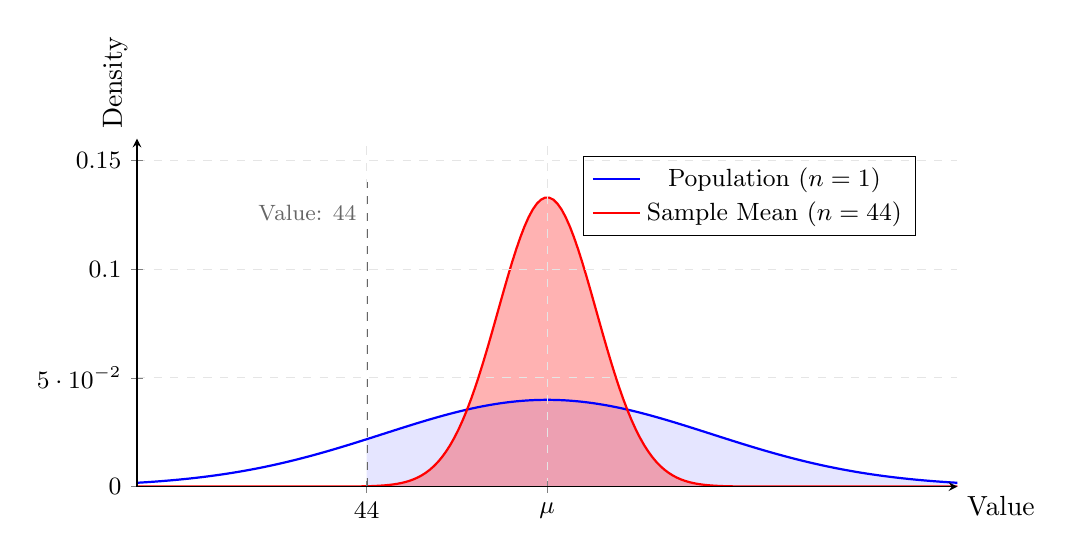
\begin{tikzpicture}
\begin{axis}[
    no markers,
    domain=30:80,
    samples=200,
    ymin=0, ymax=0.16,
    axis lines=left,
    width=12cm,
    height=6cm,
    xlabel={Value},
    ylabel={Density},
    xlabel style={at={(ticklabel* cs:1)}, anchor=north west, font={\figurelatinfont}},
    ylabel style={at={(ticklabel* cs:1)}, anchor=south west, font={\figurelatinfont}},
    tick label style={font={\figurelatinfont}\small},
    legend style={at={(0.95,0.95)}, anchor=north east, font={\figurelatinfont}\small},
    xtick={44, 55},
    xticklabels={44, $\mu$},
    enlargelimits=false,
    clip=true,
    axis on top,
    grid = major,
    grid style={dashed, gray!20}
]
\def\gauss#1#2{1/(#2*sqrt(2*pi))*exp(-((x-#1)^2)/(2*#2^2))}
\def\mval{55}
\addplot [name path=pop, blue, thick] {\gauss{\mval}{10}};
\addlegendentry{Population ($n=1$)}
\addplot [name path=sample, red, thick] {\gauss{\mval}{3}};
\addlegendentry{Sample Mean ($n=44$)}
\path[name path=axis] (axis cs:30,0) -- (axis cs:80,0);
\addplot [fill=blue, fill opacity=0.1] fill between [of=pop and axis, soft clip={domain=44:80}];
\addplot [fill=red, fill opacity=0.3] fill between [of=sample and axis, soft clip={domain=44:80}];
\draw [dashed, thick, black!60] (axis cs:44,0) -- (axis cs:44,0.14) node[pos=0.9, left, font=\footnotesize] {Value: 44};
\end{axis}
\end{tikzpicture}
\end{document}
